\documentclass[border=0pt]{standalone}
\usepackage{amsmath,graphicx}
\newcommand{\figurelabel}{\fontsize{9}{11}\selectfont}
\newcommand{\paneltitle}[2]{{\fontsize{10}{12}\selectfont\textbf{(#1)}\enspace #2}}
\begin{document}
% Both images use the same projection and pixel-to-print scale.
% Coordinates are in original render pixels, with y increasing downward.
\setlength{\unitlength}{0.245pt}
\newcommand{\atpixel}[4]{\put(\numexpr#1-145\relax,\numexpr#2-#3\relax){#4}}
\newcommand{\localpixel}[3]{\atpixel{#1+305}{2450}{#2}{#3}}
\begin{picture}(2065,2155)
  % Panel (a). The first y argument is the panel's baseline in render coordinates.
  \localpixel{0}{1500}{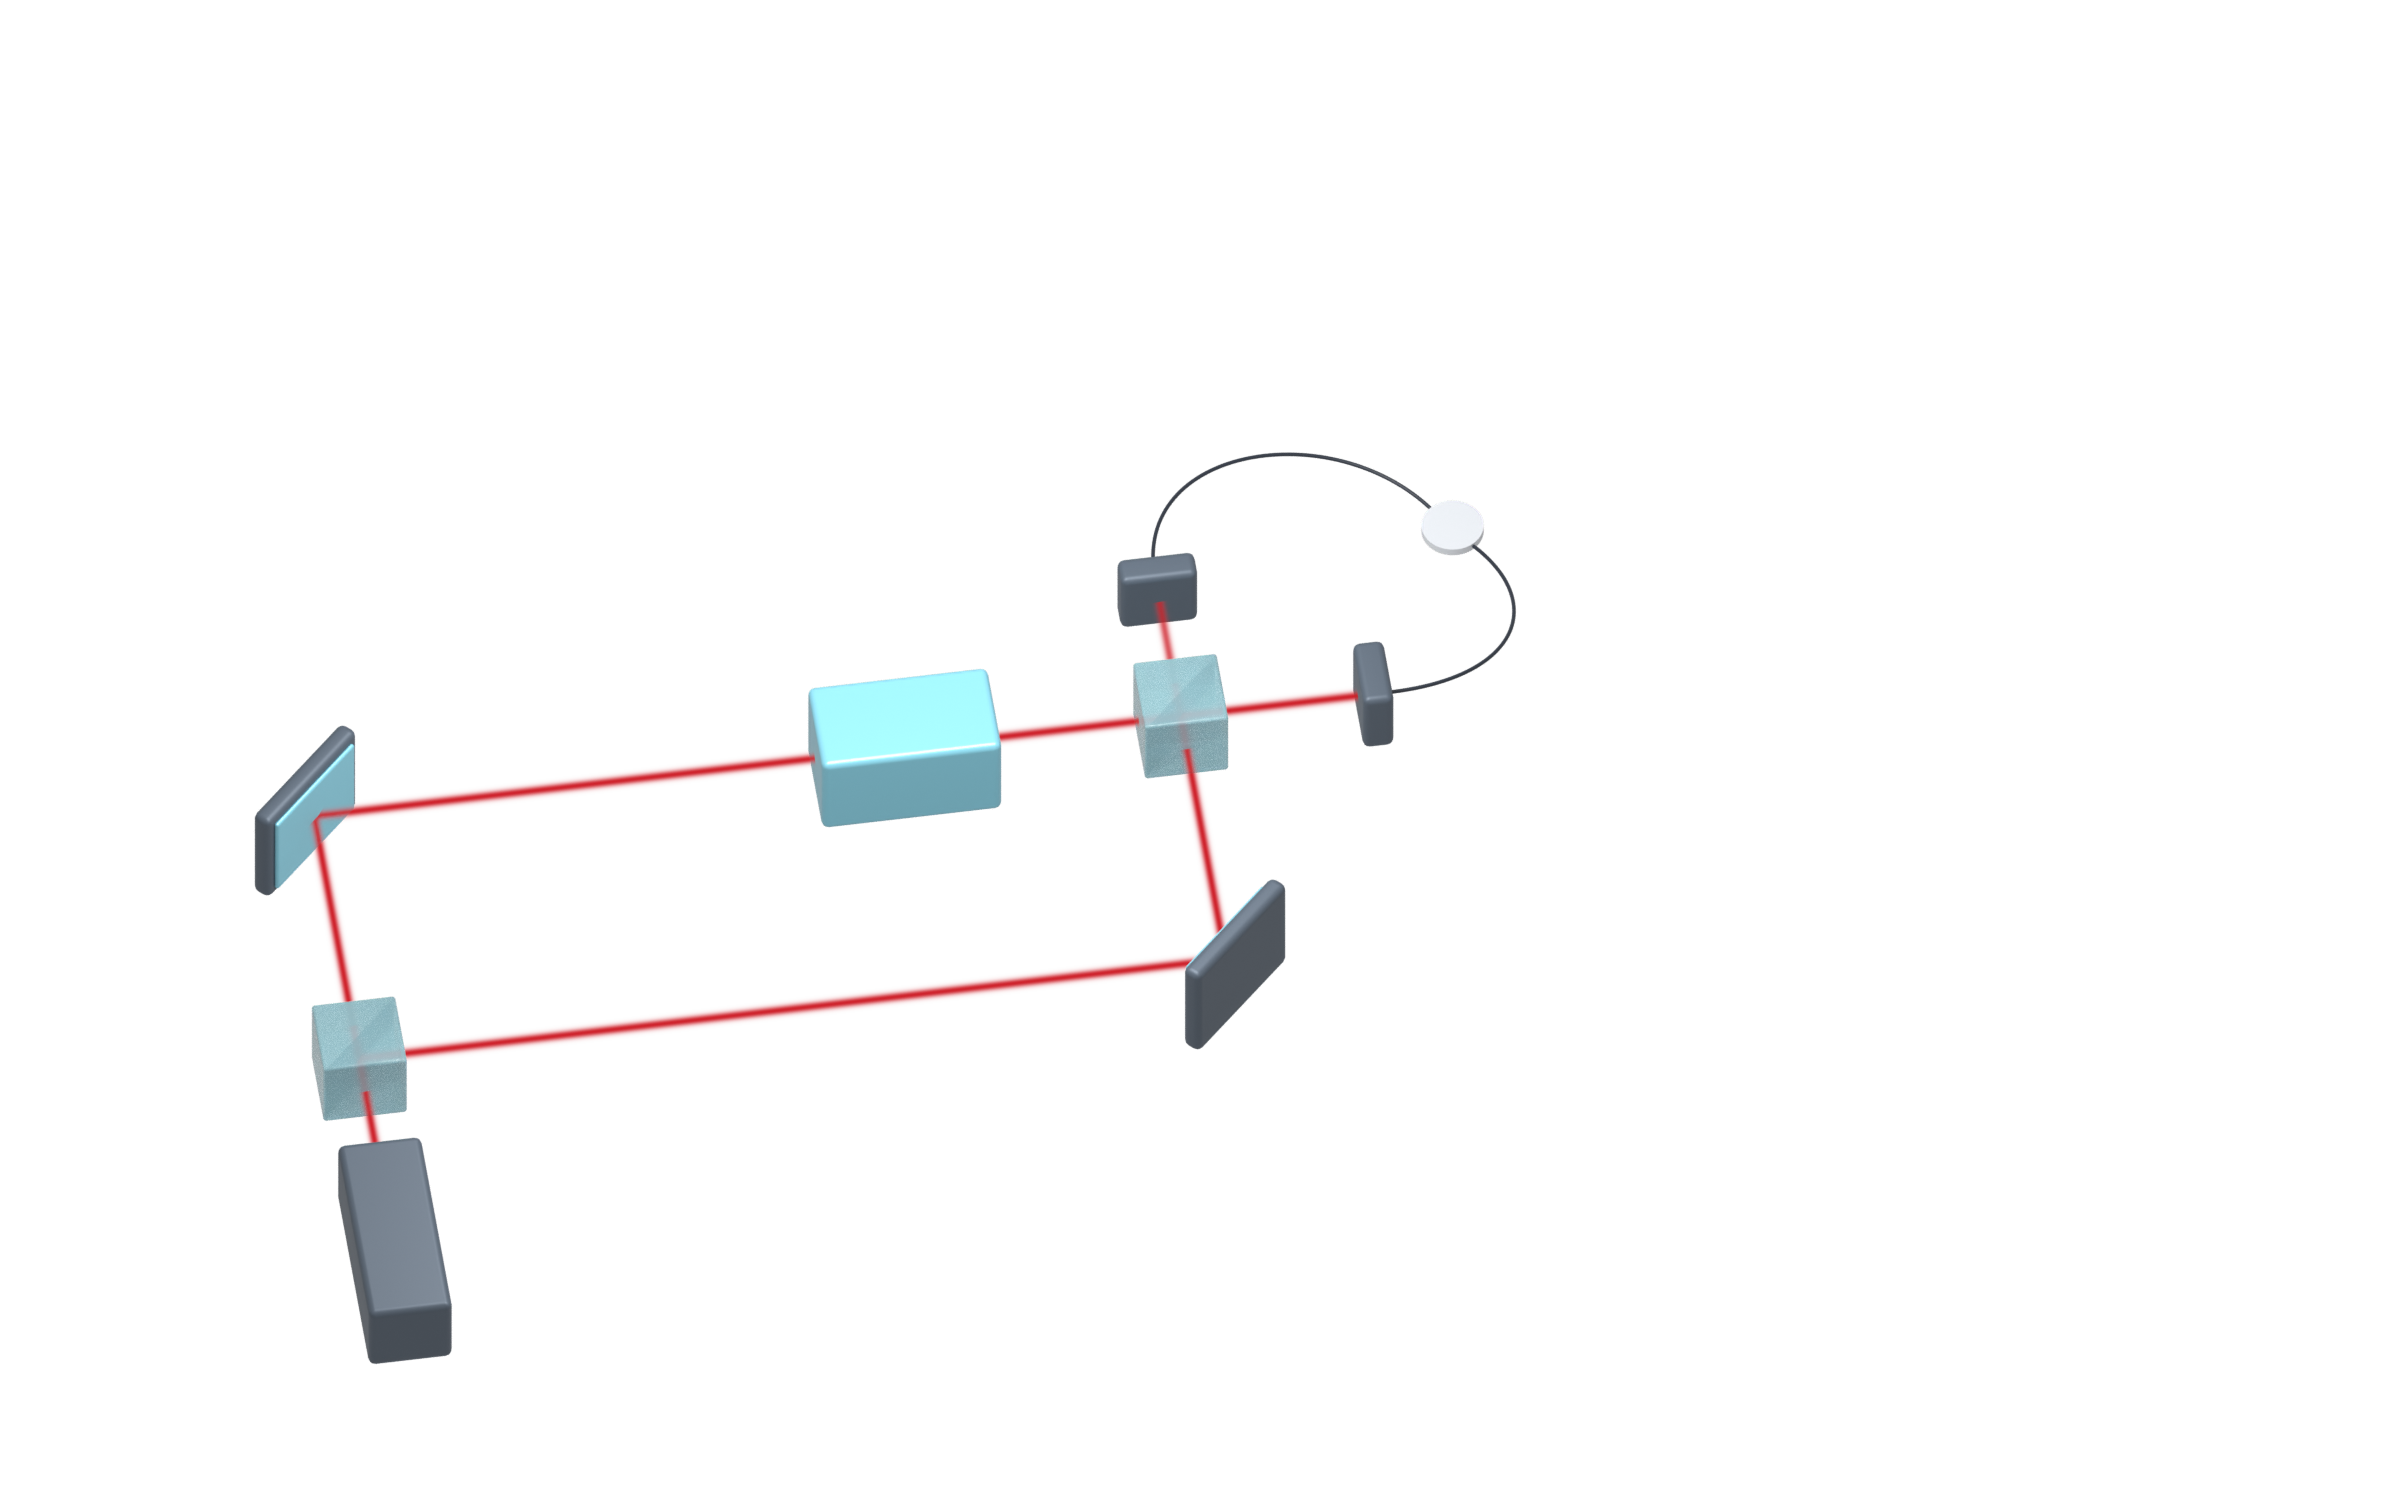
\includegraphics[width=588pt]{local_characterization.png}}
  \atpixel{158}{2450}{372}{\paneltitle{a}{Local characterization}}
  \localpixel{189}{1275}{\figurelabel Laser}
  \localpixel{243}{700}{\figurelabel Pump SLM}
  \localpixel{456}{715}{\figurelabel $(p=0,\ell_0,w)+\mathrm{seed}$}
  \localpixel{908}{793}{\makebox(0,0){\figurelabel $\chi^{(3)}$}}
  \localpixel{1140}{405}{\figurelabel Homodyne detection}
  \localpixel{1200}{1075}{\figurelabel LO SLM}
  \localpixel{1263}{841}{\figurelabel $v$}
  \localpixel{1453}{524}{\makebox(0,0){\figurelabel $-$}}

  % Panel (b).
  \atpixel{0}{1240}{1500}{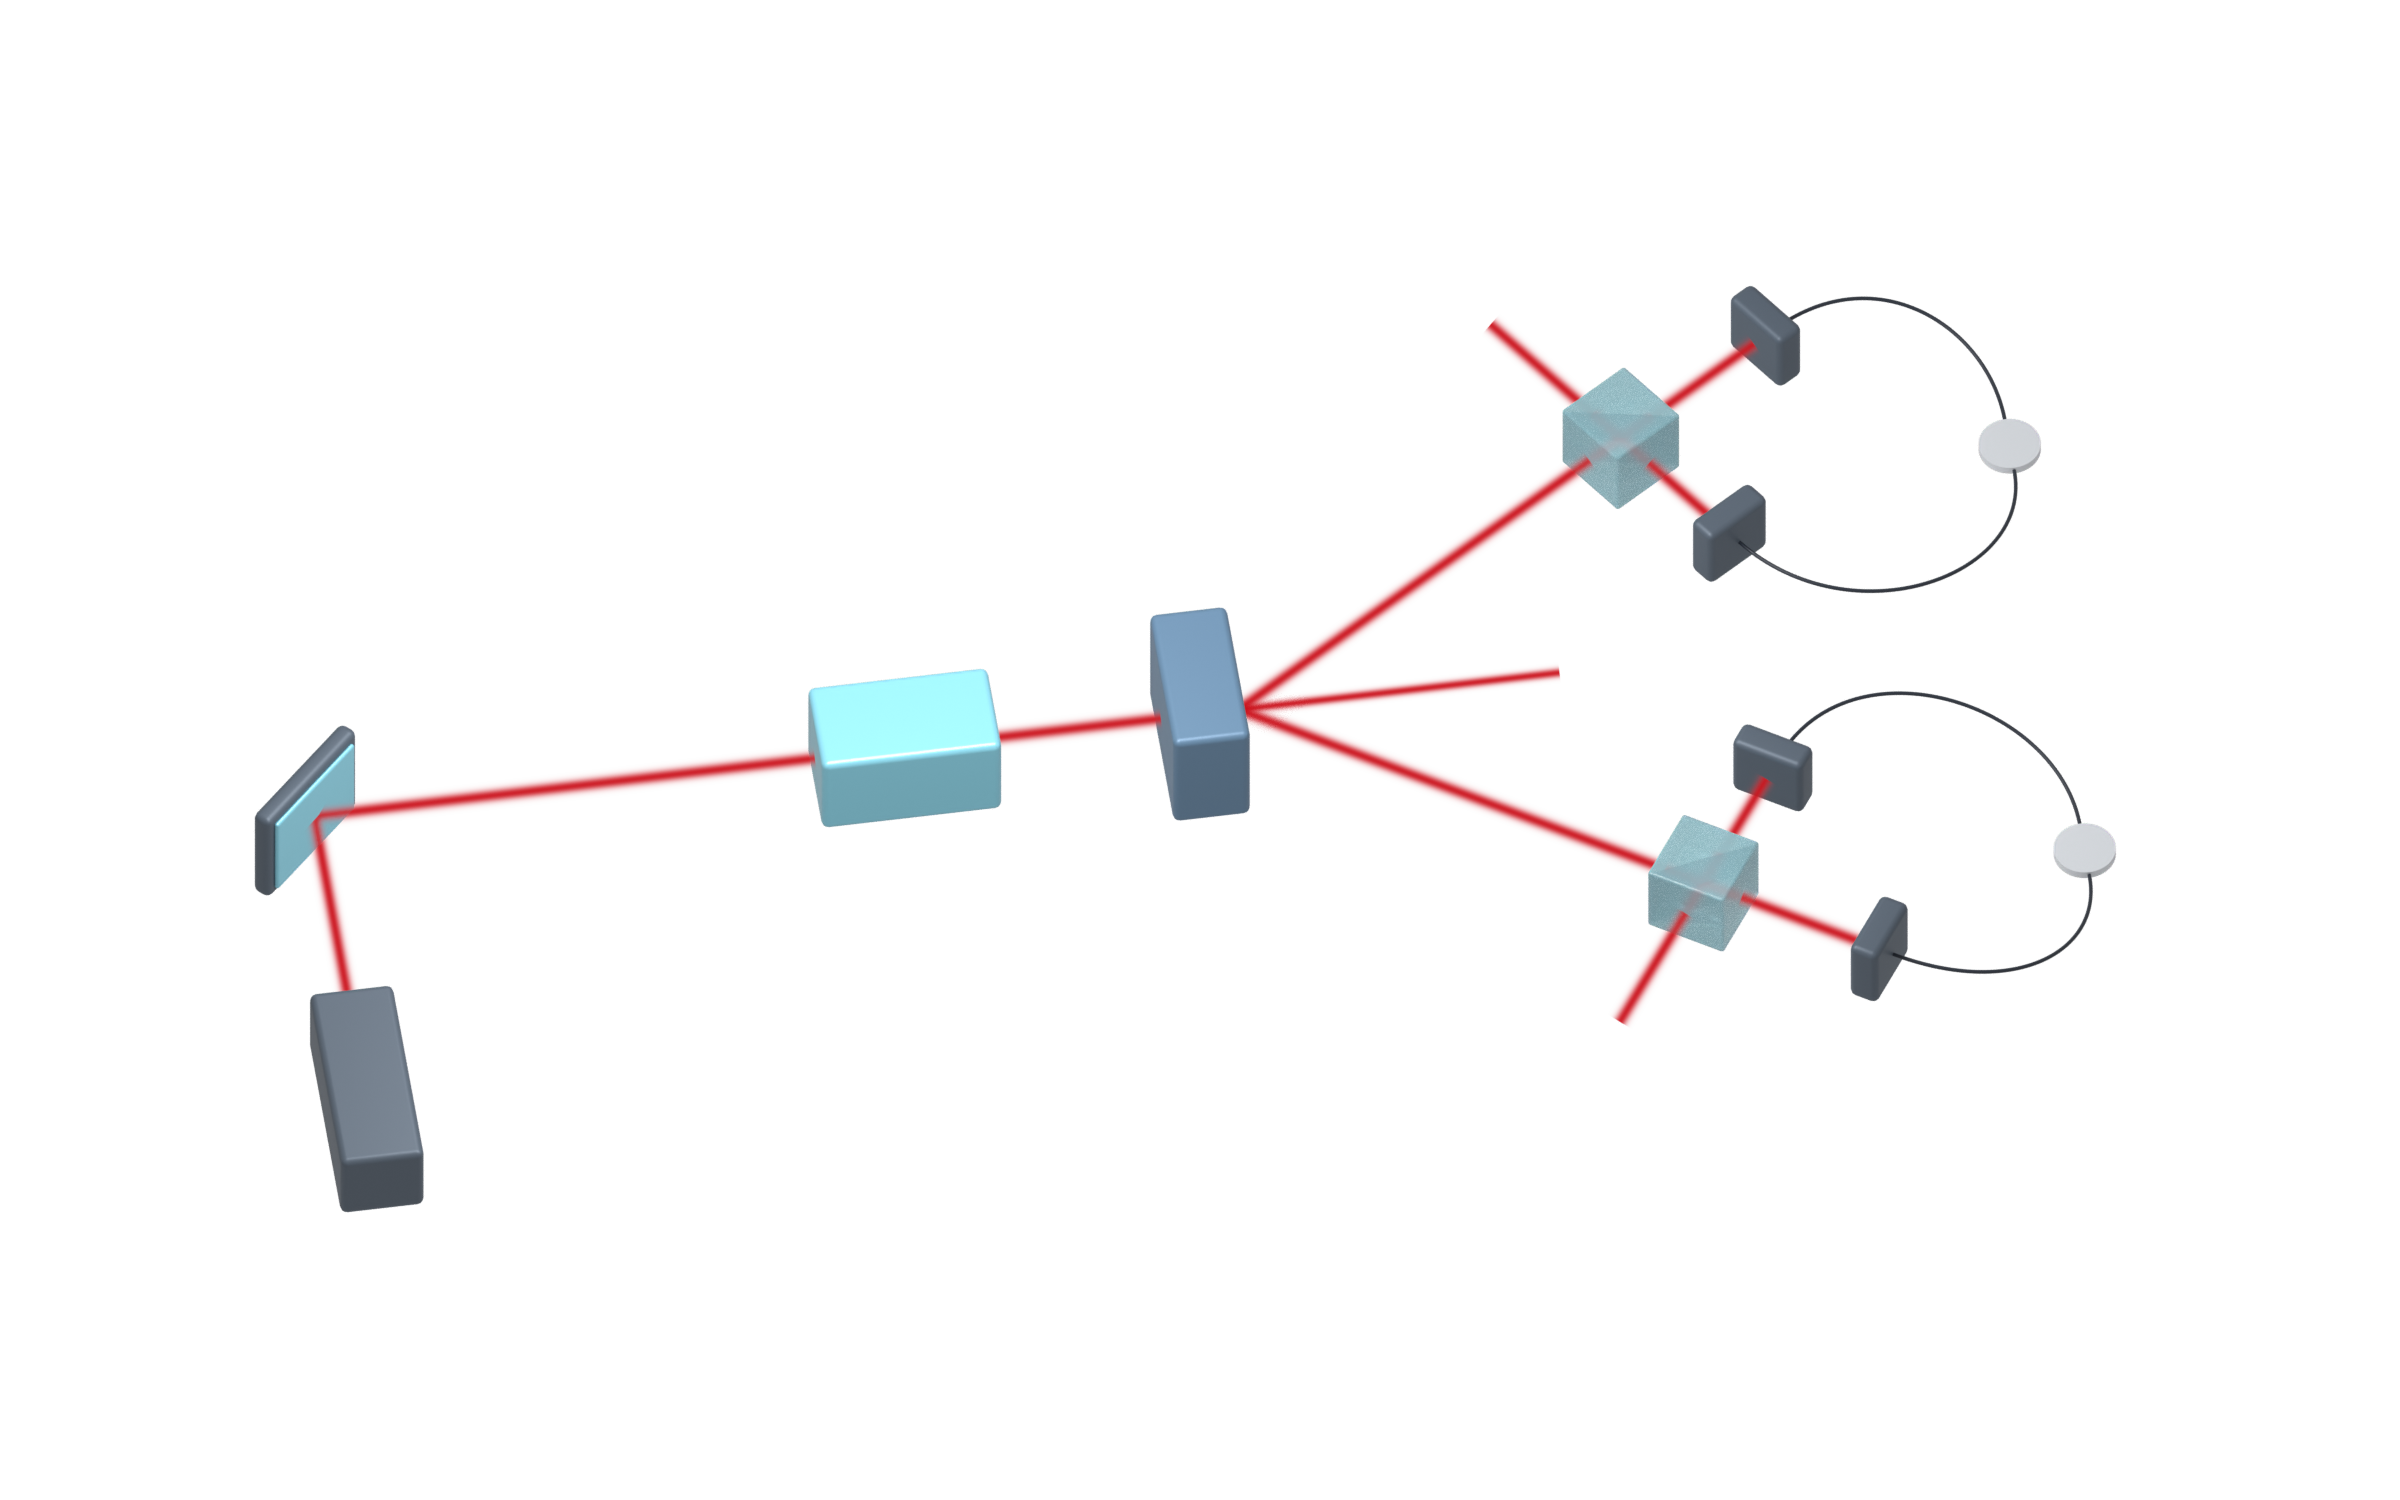
\includegraphics[width=588pt]{mode_distribution.png}}
  \atpixel{158}{1240}{214}{\paneltitle{b}{Mode distribution}}
  \atpixel{161}{1240}{1120}{\figurelabel Laser}
  \atpixel{243}{1240}{700}{\figurelabel Pump SLM}
  \atpixel{456}{1240}{715}{\figurelabel $(p=0,\ell_0,w)+\mathrm{seed}$}
  \atpixel{908}{1240}{793}{\makebox(0,0){\figurelabel $\chi^{(3)}$}}
  \atpixel{1110}{1240}{583}{\figurelabel LG sorter}
  \atpixel{1348}{1240}{555}{\figurelabel $\mathcal{B}_0$}
  \atpixel{1413}{1240}{859}{\figurelabel $\mathcal{A}$}
  \atpixel{1369}{1240}{271}{\figurelabel $\mathrm{LO}_{\mathcal{B}_0}$}
  \atpixel{1530}{1240}{1096}{\figurelabel $\mathrm{LO}_{\mathcal{A}}$}
  \atpixel{1590}{1240}{679}{\figurelabel $\dots$ additional modes}
  \atpixel{2009}{1240}{444}{\makebox(0,0){\figurelabel $-$}}
  \atpixel{2084}{1240}{847}{\makebox(0,0){\figurelabel $-$}}
\end{picture}
\end{document}
